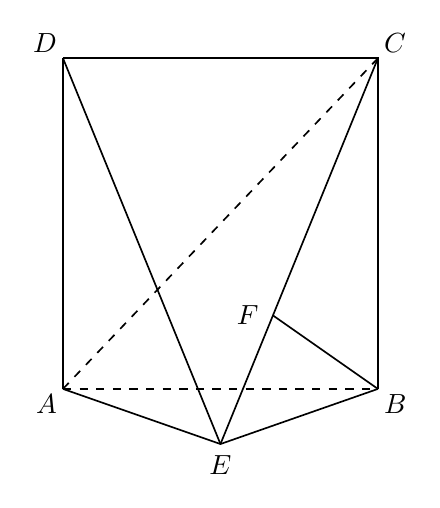
\begin{tikzpicture}[x=1cm,y=1cm,font=\normalsize,
 geometry edge/.style={solid,line width=.6pt},
 geometry label/.style={font=\normalsize,inner sep=2pt}]
\coordinate (D) at (0,4.2);
\coordinate (C) at (4,4.2);
\coordinate (A) at (0,0);
\coordinate (B) at (4,0);
\coordinate (E) at (2,-0.7);
\coordinate (F) at (2.666666667,0.9333333333);
\draw[geometry edge] (D)--(C)--(B);
\draw[geometry edge] (D)--(A);
\draw[geometry edge] (D)--(E);
\draw[geometry edge] (C)--(F)--(E);
\draw[geometry edge] (F)--(B);
\draw[geometry edge] (B)--(E)--(A);
\draw[geometry edge,dashed] (A)--(B);
\draw[geometry edge,dashed] (A)--(C);
\node[geometry label,above left] at (D) {$D$};
\node[geometry label,above right] at (C) {$C$};
\node[geometry label,below left] at (A) {$A$};
\node[geometry label,below right] at (B) {$B$};
\node[geometry label,below,yshift=-2pt] at (E) {$E$};
\node[geometry label,left,xshift=-3pt] at (F) {$F$};
\end{tikzpicture}
